
\subsection*{1.}

En dérivant le produit, toutes les fonctions étant dérivables :
\[
f'(x) = 2 e^x + (2x - 1) e^x = e^x(2 + 2x - 1) = (2x + 1) e^x.
\]

\subsection*{2.}

On sait que, quel que soit \(x \in \mathbb{R}\), \(e^x > 0\) : le signe de \(f'(x)\) est celui de \(2x + 1\) qui s'annule pour :
\[
2x + 1 = 0 \quad \Longleftrightarrow \quad x = -\dfrac{1}{2}.
\]
On en déduit :
\begin{itemize}
    \item \(f'(x) > 0\) sur l'intervalle \(\left]-\dfrac{1}{2}\,;\,+\infty\right[\) ;
    \item \(f'(x) < 0\) sur l'intervalle \(\left]-\infty\,;\,-\dfrac{1}{2}\right[\).
\end{itemize}

\subsection*{3.}

La question précédente montre que la fonction \(f\) est décroissante sur l'intervalle \(\left]-\infty\,;\,-\dfrac{1}{2}\right[\), et croissante sur l'intervalle \(\left]-\dfrac{1}{2}\,;\,+\infty\right[\), avec un minimum en \(x = -\dfrac{1}{2}\), où :
\[
f\left(-\dfrac{1}{2}\right) = \left(2 \times \left(-\dfrac{1}{2}\right) - 1\right) e^{-\frac{1}{2}} = -2 e^{-\frac{1}{2}} \approx -1,213.
\]
D'où le tableau de variations sur \(\mathbb{R}\) :

\begin{center}
\begin{tikzpicture}
\tkzTabInit[lgt=3.5, espcl=3]{$x$ / 1, {Signe de $f'(x)$} / 1, {$f$} / 2}{${-\infty}$, ${-\dfrac{1}{2}}$, ${+\infty}$}
\tkzTabLine{,-,0,+,}
\tkzTabVar{+/{$$},-/{$\approx -1,213$},+/{$$}}{/}
\end{tikzpicture}
\end{center}

\subsection*{4.}

\(C\) coupe l'axe des ordonnées en des points dont l'ordonnée est nulle, donc tels que :
\[
(2x - 1) e^x = 0 \quad \Longleftrightarrow \quad 2x - 1 = 0 \quad (\text{car } e^x \neq 0) \text{ d'où } x = \dfrac{1}{2}.
\]

\(C\) coupe l'axe des ordonnées au point \(\left(\dfrac{1}{2}\,;\,0\right)\).

\subsection*{5.}

\(M(x\,;\,y) \in T \Longleftrightarrow y - f(0) = f'(0)(x - 0).\)

Avec \(f(0) = -e^0 = -1\) et \(f'(0) = 1e^0 = 1\), on obtient :

\(M(x\,;\,y) \in T \Longleftrightarrow y - (-1) = 1(x - 0) \Longleftrightarrow y = x - 1.\)

